\svnid{$Id: UserInterface.tex 1 2007-12-12 17:37:26Z t-scheller $}
\section{Graphical User Interface} \label{ui:User interface}
\subsection{Package and file states} \label{ui:Package and file states}
The \gl[instrumentable item]{instrumentable items} (e.g. packages or source \gl[code file]{code files}) are presented in one of two states: \textit{normal} and \textit{used for coverage measurement}. The following table shows the icons for different instrumentable items in these states.
{\small
  \begin{longtable}{|c|c|c|c|}\hline
   {\normalsize \textbf{Object}} &
   {\normalsize \textbf{normal}} &
   {\normalsize \textbf{used for coverage measurement}} \\\hline \hline \endhead
%    {\normalsize \textbf{Instrumented}} \\\hline \hline \endhead
   Package & 
   
\includegraphics[]{images/Package_Explorer/package_symbol} &
   \includegraphics[]{images/Package_Explorer/package_select_for_instrumentation} \\\hline
%    
\includegraphics[]{images/Package_Explorer/package_instrumented} \\\hline
   Java file & 
   \includegraphics[]{images/Package_Explorer/java_file_symbol} &
   \includegraphics[]{images/Package_Explorer/java_file_select_for_instrumentation} \\\hline
%    
\includegraphics[]{images/Package_Explorer/java_file_instrumented} \\\hline
%    \caption{Package and file states}
  \end{longtable}
}
\par
The user can change the state of an instrumentable item by selecting the \eclui{Use For Coverage Measurement} menu item in the context menu of an instrumentable item (e.g. in the JDT's \eclui{Package Explorer} or the generic \eclui{Navigator}). \eclui{Use for Coverage Measurement} is a check box menu item so that a second selection of this menu item removes the instrumentable item from coverage measurement. 
 
\begin{figure}[hbtp]
 \centering
 \includegraphics[]{images/Package_Explorer/Package_Explorer}
 \caption{Package selection}
 \label{ui_fg:Package selection}
\end{figure}
\par
\subsection{Instrumentation} \label{ui:Instrumentation}
The \eclui{Instrument Project\dots} item is added to the \eclui{Project} menu. This command opens the dialog window which is shown in figure \ref{ui_fg:Instrumentation dialog}.
\begin{figure}[hbtp]
 \centering
 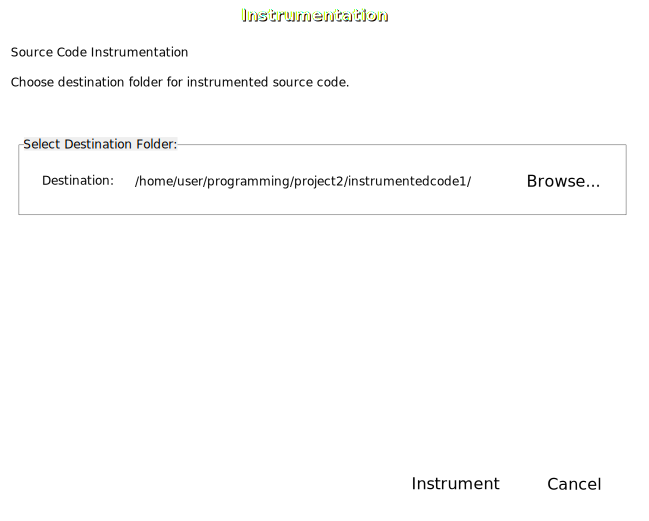
\includegraphics[width=\textwidth]{images/Instrumentation_Dialog/Instrumentation_Dialog}
 \caption{Instrumentation dialog}
 \label{ui_fg:Instrumentation dialog}
\end{figure}

\subsection{Launching} \label{ui:Launching}
The software adds a new launch mode to the Eclipse workbench. This mode is called Coverage mode and works exactly like the existing Run and Debug modes. Figure \ref{ui_fg:Coverage button} shows the pull down menu of the \eclui{Coverage Button} on the tool bar. The menu items \eclui{Coverage History}, \eclui{Coverage As} and \eclui{Coverage\dots} are added to the \eclui{Coverage} menu.
\par
The \eclui{Coverage\dots} option opens the \eclui{Coverage} dialog which is similar to the Run dialog, except that the \eclui{Run} button in that dialog is called \eclui{Coverage}.
\begin{figure}[hbtp]
 \centering
 
\includegraphics[]{images/Coverage_Button/Coverage_Button}
 \caption{Coverage button}
 \label{ui_fg:Coverage button}
\end{figure}
\par

\subsection{Coverage view}
The coverage results are presented in the \eclui{Coverage} view. It displays the results of \gl[statement]{statement}, branch, condition and \gl[loop coverage]{loop coverage} per \gl[project]{project}, package, class (including interfaces and enums) and method. This view is shown in figure \ref{ui_fg:Coverage view}.
\begin{figure}[hbtp]
 \centering
 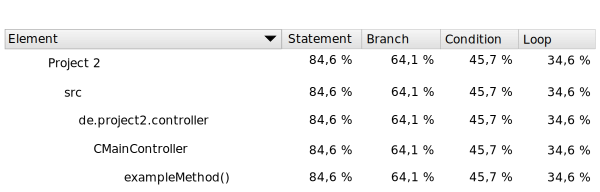
\includegraphics[]{images/Coverage_View/Coverage_View.png}
 \caption{Coverage view}
 \label{ui_fg:Coverage view}
\end{figure}
\par
A grey bar is shown left of a coverage result if there are no \gl[coverable item]{coverable items} of the associated \gl[coverage criterion]{coverage criterion} in the associated \eclui{Element}.

The check box in the upper-left corner of the view enables a simple filter if checked. If the filter is activated only methods with a coverage result smaller, smaller or equal, greater, greater or equal than a given percentage are shown in the coverage view. The coverage criterion to compare with can be selected in the most left combo box in the view. The operator to compare the coverage result with can be selected in the combo box right of the combo box of the coverage criteria. The percentage to compare with can be entered in the field right of the combo box of the comparison operators.

The tool bar items in the upper-right part of the view provide the possibility to select Java elements shown as root entries in the element column. Possible root entries are projects, packages, classes (including interfaces, enums and annotations) and methods.

\subsection{Test sessions view} \label{ui:Test sessions view}
The \eclui{Test Sessions} view lists the \gl[test session]{test sessions} of the selected \gl[session container]{session container}. Figure \ref{ui_fg:Session view} shows an example of this view. A session container can be chosen using the combo box. The session container list entries display the date and time along with the associated \gl[project]{project}.
\begin{figure}[hbtp]
 \centering
 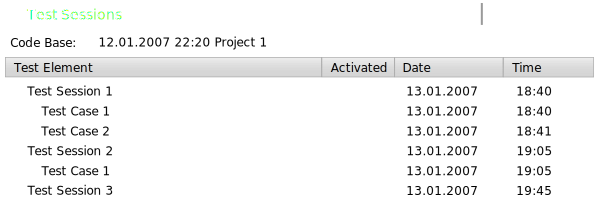
\includegraphics[]{images/Test_Case_Administration_View/Session_View.png}
 \caption{Test Sessions view}
 \label{ui_fg:Session view}
\end{figure}
\par
The check box in front of each row determines whether a \eclui{Test Element} is activated. The coverage results of activated \eclui{Test Element}s are visualized by the views of the plugin (e.g., \eclui{Coverage} view) and the source code highlighting. The visualizations are automatically refreshed as the user activates or deactivates particular \eclui{Test Element}s. By default, all \eclui{Test Element}s are activated.
\par
The activation or deactivation of a test session activates or deactivates all test cases of this test session. For test sessions the check box has an additional state, partly activated. This state is visualized by the crossed out check box in figure \ref{ui_fg:Session view} and means that at least one test case of a selected test session is deactivated. 
\par
The information about the set of active (visualized) \eclui{Test Element}s is stored; that is, selecting a new session container does not change the set of the active \eclui{Test Element}s of the previous session container.
\par
The tool bar items represent following commands (from left to right):
\begin{itemize}
\item Delete Test Session Container
  \begin{itemize}
  \item Delete Multiple Containers
  \end{itemize}
\item Merge
\item Delete
\end{itemize}
\eclui{Delete Test Session Container} deletes the active session container. Prior to the actual deletion the user has to confirm his intent to do so. By using the drop-down menu of the \eclui{Delete Session Container} item, the user can reveal the item for the deletion of multiple session containers: \eclui{Delete Multiple Containers}. It opens a dialog that prompts the user to select the session containers to delete and performs the deletion after the user confirmed the selection.  The item \eclui{Merge} allows the user to merge the selected test elements. On selection of this item a dialog pops up which prompts the user to select the type of test element (test cases or test sessions) to merge and prompts the user to enter a name and comment for the merged test element. Furthermore the user is able to review and change the set of test elements to merge. The \eclui{Delete} item deletes the selected test elements, whereas the user is asked for confirmation before the deletion is performed.
\par
The \eclui{Test Element}s have a context menu which contains following items:
\begin{itemize}
\item Select All
\item Activate All
\item Deactivate All
\item Delete
\item Properties
\end{itemize}
The item \eclui{Select All} selects all test elements of the active session container to be able to delete them all at once for example. \eclui{Activate All} and \eclui{Deactivate All} activate or respectively deactivate all test elements of the active session container. The item \eclui{Delete} evokes the same action as described above. The \eclui{Properties} item opens a dialog which allows the user to edit the properties of the selected \eclui{Test Element}. The \eclui{Test Case Properties} dialog is shown in figure \ref{ui_fg:Test case properties}. It is possible to change the name of the selected \eclui{Test Element}. Furthermore, a multi line comment may be entered.
\begin{figure}[hbtp]
 \centering
 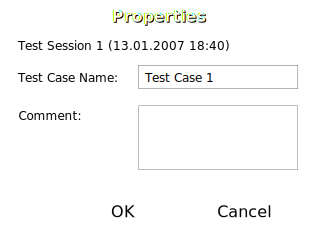
\includegraphics[width=0.5\textwidth]{images/Test_Case_Administration_View/Test_Case_Properties.png}
 \caption{Test case properties}
 \label{ui_fg:Test case properties}
\end{figure}

\subsection{Import} \label{ui:Import}
The software extends the standard Eclipse \eclui{Import} interface by adding two entries to group \eclui{\gbt}, \eclui{Test Session Container} and \eclui{\gbt Coverage Log}. Figure \ref{ui_fg:Import Test Session Container} shows the correspondent \eclui{Import} wizard page. This dialog allows the user to select a \gl[session container]{session container} and a \gl[project]{project} into which the session container will be imported. The file extensions used in the following dialogs are examples.
\begin{figure}[hbtp]
 \centering
 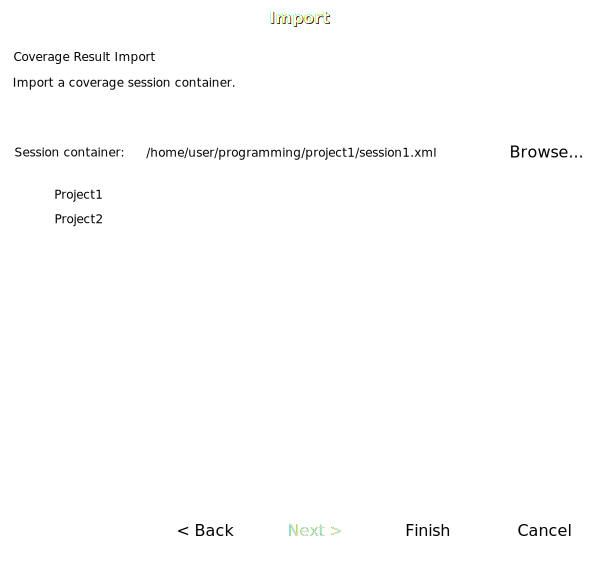
\includegraphics[width=0.85\textwidth]{images/Test_Case_Administration_View/Import_Session.png}
 \caption{Import Test Session Container}
 \label{ui_fg:Import Test Session Container}
\end{figure}
\par
Selecting \eclui{\gbt Coverage Log} proceeds with the wizard page shown in figure \ref{ui_fg:Import Coverage Log}. This import operation requires the \gl[coverage log]{coverage log} file, created while running the instrumented program. Moreover the user has to select the session container the coverage log will be imported to and enter a name and comment for the new test session that will contain the data of the coverage log.
\begin{figure}[hbtp]
 \centering
 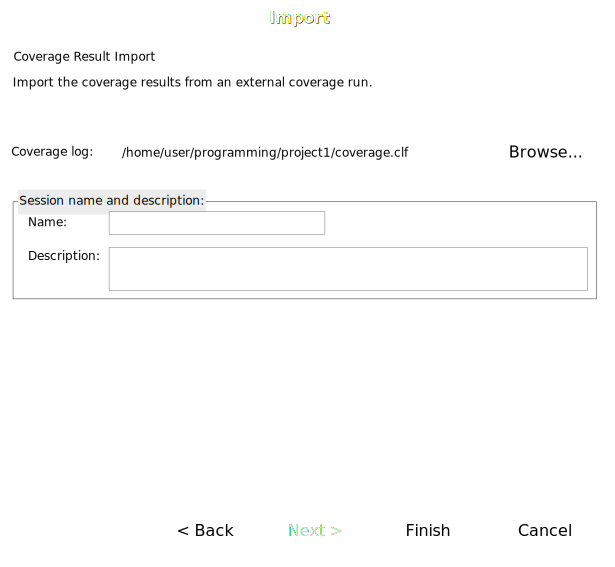
\includegraphics[width=0.9\textwidth]{images/Test_Case_Administration_View/Import_Coverage_Log.png}
 \caption{Import Coverage Log}
 \label{ui_fg:Import Coverage Log}
\end{figure}
\par

\subsection{Export} \label{ui:Export}
The item \eclui{\gbt Coverage Result Export} is added to the \eclui{Other} group of standard Eclipse \eclui{Export} dialog. The respective wizard page is shown in figure \ref{ui_fg:Export Test Session}. The dialog contains the list of all available \gl[test session]{test sessions} in the selected code base. The list \eclui{Available Test Sessions} allows multiple selections. The code base can be chosen from the combo box. By default, the last code base or the code base which is used in the \eclui{Test Sessions} view is preselected.
\begin{figure}[hbtp]
 \centering
 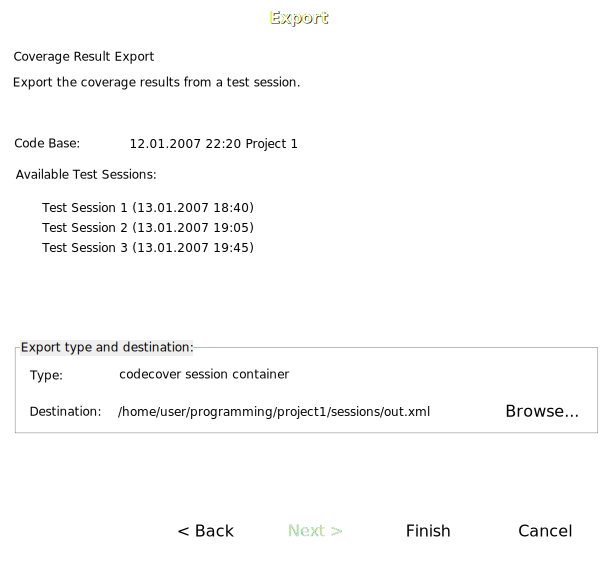
\includegraphics[]{images/Test_Case_Administration_View/Export_Session}
 \caption{Export Test Session}
 \label{ui_fg:Export Test Session}
\end{figure}
\par
Possible export types are \eclui{\gbt Session Container} and \textit{Report}. The report type has an extra wizard page which allows the user to select a report template (figure \ref{ui_fg:Report dialog}).
\begin{figure}[hbt]
 \centering
 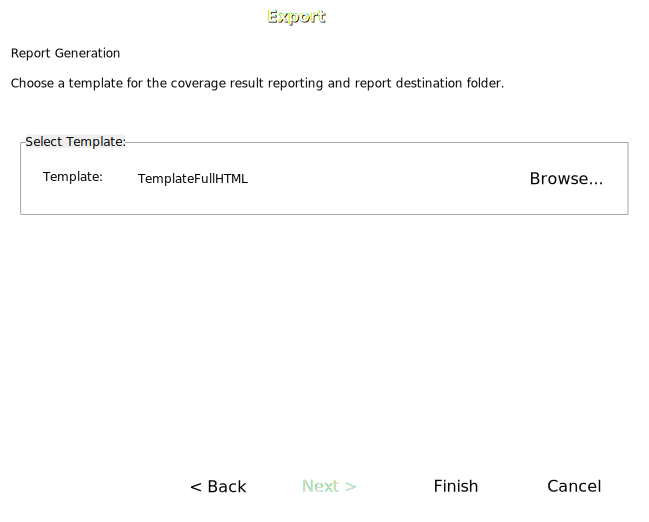
\includegraphics[width=1.0\textwidth]{images/Report_Configuration_Dialog/Report_Configuration_Dialog}
 \caption{Report dialog}
 \label{ui_fg:Report dialog}
\end{figure}
\par

\subsection{Source code highlighting} \label{ui:Source code highlighting}
\subsubsection{General}
This section describes the visualization of coverage results by highlighting  the source code of the \gl[SUT]{SUT}. There are three different colors for displaying the state of a particular part of code. The default color scheme uses green for ``covered'', yellow for ``partly covered'' and red for ``not covered''. All these colors are configurable (see section~\ref{ui:Preferences dialog}). Throughout this section, the default colors are used to explain the details of the highlighting. 

Statement coverage is shown by highlighting the \gl[statement]{statements}. To display \gl[branch coverage]{branch coverage}, the keywords of \gl[conditional statement]{conditional statements} are highlighted. Condition coverage is represented by coloring each basic term of a condition with green or red. For \gl[loop coverage]{loop coverage}, the keywords of looping statements are highlighted. All examples in this section show source code highlighting with all coverage criteria.
\subsubsection{Java}

\paragraph{Basic statements}
Basic statements are completely highlighted either green or red, for covered and not covered statements, respectively.

\paragraph{Conditional statements}
\subparagraph{If-then-else statements}
The following list describes the meaning of the background color of the \texttt{if} keyword:
\begin{itemize}
\item \textbf{Green:}  Both branches are covered.
\item \textbf{Yellow:}  Only the then-branch is covered.
\item \textbf{Red:}  Only the else-branch is covered.
\end{itemize}
\par
Figure \ref{ui_fg:If-then statements} illustrates the different possibilities of if-then coverage. If the branching statement is not evaluated because it is not executed, it is also highlighted with red color.
\begin{figure}[hbt]
 \hfill
 \includegraphics[]{images/Source_Code_Highlighting/if/if_without_else_green}
 \hfill
 \includegraphics[]{images/Source_Code_Highlighting/if/if_without_else_yellow}
 \hfill
 \includegraphics[]{images/Source_Code_Highlighting/if/if_without_else_red}
 \hspace{1cm}
 \hfill
 \caption{If-then statements}
 \label{ui_fg:If-then statements}
\end{figure}
\par
The background color of \texttt{else} keyword has the following meanings:
\begin{itemize}
\item \textbf{Green:}  The else-branch is covered.
\item \textbf{Red:}  The else-branch is not covered.
\end{itemize}
\par
\begin{figure}[hbt]
 \hfill
 \includegraphics[]{images/Source_Code_Highlighting/if/if_with_else_green}
 \hfill
 \includegraphics[]{images/Source_Code_Highlighting/if/if_with_else_yellow}
 \hfill
 \includegraphics[]{images/Source_Code_Highlighting/if/if_with_else_red-green}
 \hspace{1cm}
 \hfill
 \caption{If-then-else statements}
 \label{ui_fg:If-then-else statements}
\end{figure}
\par
Example highlighting of if-then-else statements is shown in the figure  \ref{ui_fg:If-then-else statements}. The left picture represents full statement, branch and \gl[condition coverage]{condition coverage}. In the middle picture only the then-branch and in the right one only the else-branch is covered. 
\par
An if-then-else statement can be nested in another if-then-else statement. In that case the same color scheme as described above is applied. Figure \ref{ui_fg:Nested if-then-else statements} shows some examples for nested if-then-else statements.
\begin{figure}[htp]
 \hfill
 \includegraphics[]{images/Source_Code_Highlighting/if/if_with_else_if_green-yellow}
 \hfill
 \includegraphics[]{images/Source_Code_Highlighting/if/if_with_else_if_red-green-red}
 \hfill
 \includegraphics[]{images/Source_Code_Highlighting/if/if_with_else_if_yellow}
 \hfill
 \caption{Nested if-then-else statements}
 \label{ui_fg:Nested if-then-else statements}
\end{figure}
\par

\subparagraph{Switch statements}
The following list describes the highlighting scheme for the \texttt{switch} keyword:
\begin{itemize}
\item \textbf{Green:}  All cases are covered.
\item \textbf{Yellow:}  Some cases are covered, but at least one case is not covered.
\item \textbf{Red:}  No case is covered.
\end{itemize}
If the default section of the \texttt{switch} statement is not covered the \texttt{switch} keyword is highlighted as partly covered (yellow) as well. The highlighting is independent from the fact that the default section can be omitted. Figure \ref{ui_fg:Switch-statement with some cases and default section} shows a sample highlighted \texttt{switch} statement with a \texttt{default} section.
\par
For every case the keyword \texttt{case} and the \texttt{constant} are highlighted the following:
\begin{itemize}
\item \textbf{Green:}  The case is covered.
\item \textbf{Red:}  The case is not covered.
\end{itemize}
If the default section is not omitted, the keyword \texttt{default} is highlighted the same way as cases.

\begin{figure}[hbt]
 \centering
 \includegraphics[]{images/Source_Code_Highlighting/switch/switch}
 \caption{Switch-statement with some cases and a default section}
 \label{ui_fg:Switch-statement with some cases and default section}
\end{figure}
\par
\par

\paragraph{Looping statements}
\subparagraph{General}
The keywords of looping statements (\texttt{while}, \texttt{for} and \texttt{do-while}) are highlighted as specified in the following list. The \gl[loop coverage]{loop coverage} is defined in section \ref{fr:Loop coverage}.
\begin{itemize}
\item \textbf{Green:}  Loop body is covered (fulfill all requirements of loop coverage). 
\item \textbf{Yellow:}  Loop body is partly covered (at least one requirement of loop coverage, but not all requirements).
\item \textbf{Red:}  Loop body is not covered at all.
\end{itemize}
\par

\subparagraph{While loops}
Figure \ref{ui_fg:While statements} shows full, partly and not covered \texttt{while} loops (from left to right).
\begin{figure}[hbt]
 \hfill
 \includegraphics[]{images/Source_Code_Highlighting/while/while_green}
 \hfill
 \includegraphics[]{images/Source_Code_Highlighting/while/while_yellow}
 \hfill
 \includegraphics[]{images/Source_Code_Highlighting/while/while_red}
 \hfill
 \caption{Highlighting of while loops}
 \label{ui_fg:While statements}
\end{figure}
\par

\subparagraph{Do-while}
Do-while loop is represented similar to the \texttt{while} loop; only the \texttt{while} keyword is highlighted. The colors are the same (see figure \ref{ui_fg:Do-while statements}).
\begin{figure}[hbt]
 \hfill
 \includegraphics[]{images/Source_Code_Highlighting/do-while/do-while_green}
 \hfill
 \includegraphics[]{images/Source_Code_Highlighting/do-while/do-while_yellow}
 \hspace{2cm}
 \caption{Do-while statements}
 \label{ui_fg:Do-while statements}
\end{figure}
\par

\subparagraph{For}
The coverage results of \texttt{for} loops are visualized in the same way as those for \texttt{while} loops. Samples of highlighted \texttt{for} loops are shown in the figure \ref{ui_fg:For statements}.
\begin{figure}[hbt]
 \hfill
 \includegraphics[]{images/Source_Code_Highlighting/for/for_green}
 \hfill
 \includegraphics[]{images/Source_Code_Highlighting/for/for_yellow}
 \hfill
 \newline
 \centering
 \includegraphics[]{images/Source_Code_Highlighting/for/for_red}
 \caption{For statements}
 \label{ui_fg:For statements}
\end{figure}
\par

\subsubsection{COBOL}
\paragraph{Basic statements}
Basic statements like \texttt{DISPLAY}, \texttt{ACCEPT} or \texttt{COMPUTE} are highlighted with green and red for covered and not covered statements, respectively.

\paragraph{Conditional statements}
\subparagraph{If-then-else statements}
The highlighting scheme for if-then-else statements is completely analogous to that of the corresponding statements in Java described above. Figure \ref{ui_fg:If-then statements in COBOL} shows the highlighting of an if-then statement in the COBOL programming language:
\begin{figure}[htp]
 \hfill
 \includegraphics[]{images/Source_Code_Highlighting/if_cobol/if_without_else_green}
 \hfill
 \includegraphics[]{images/Source_Code_Highlighting/if_cobol/if_without_else_yellow}
 \hfill
 \includegraphics[]{images/Source_Code_Highlighting/if_cobol/if_without_else_red}
 \hspace{1cm}
 \hfill
 \caption{If-then statements in COBOL}
 \label{ui_fg:If-then statements in COBOL}
\end{figure}
\par

\subparagraph{Evaluate statement}
The \texttt{EVALUATE} statement is the counterpart of the Java \texttt{switch} statement. Therefore analogous highlighting rules are applied for this statement. Figure \ref{ui_fg:Evaluate statement} shows an example of the \texttt{EVALUATE} statement highlighting:
\begin{figure}[htp]
 \centering
 \includegraphics[]{images/Source_Code_Highlighting/evaluate/evaluate}
 \caption{Evaluate statement}
 \label{ui_fg:Evaluate statement}
\end{figure}
\par

\paragraph{Looping statements}
\subparagraph{Perform}
The \texttt{PERFORM} statement is overloaded and can be used as a \gl[basic statement]{basic statement} to jump to a particular paragraph (e.g. as in figure \ref{ui_fg:Evaluate statement}) as well as a loop statement. Figure \ref{ui_fg:Perform statement with test before} shows a while-equivalent statement and figure \ref{ui_fg:Perform statement with test after} a do-while-equivalent one. The highlighting rules for the while and do-while loops in Java apply accordingly. 
\begin{figure}[htp]
 \centering
 \includegraphics[]{images/Source_Code_Highlighting/perform/perform_wtb_yellow}
 \caption{Perform statement with test before}
 \label{ui_fg:Perform statement with test before}
\end{figure}
\begin{figure}[htp]
 \centering
 \includegraphics[]{images/Source_Code_Highlighting/perform/perform_wta_yellow}
 \caption{Perform statement with test after}
 \label{ui_fg:Perform statement with test after}
\end{figure}
\par

\subsection{Preferences dialog} \label{ui:Preferences dialog}
The \gbt entry in the \eclui{Preferences} dialog contains Eclipse-wide options for configuring the software. This dialog page is shown in figure \ref{ui_fg:Preferences dialog}.
\begin{figure}[hbt]
 \centering
 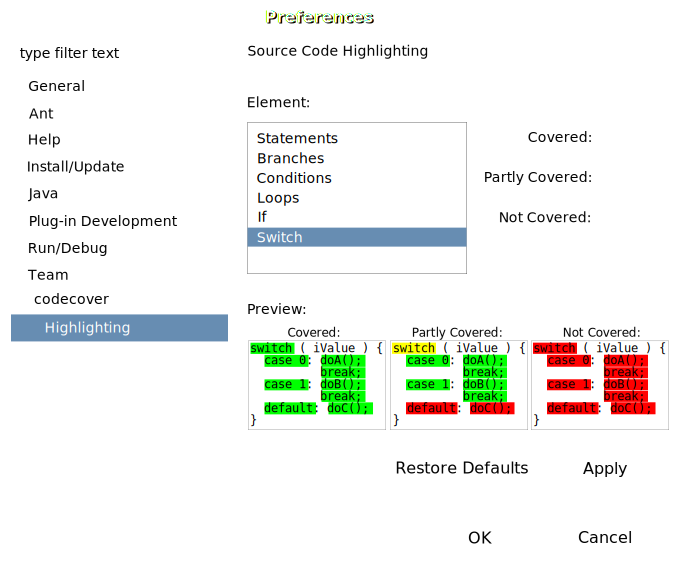
\includegraphics[width=1.0\textwidth]{images/Preferences_Highlighting/Preferences_Highlighting}
 \caption{Preferences dialog}
 \label{ui_fg:Preferences dialog}
\end{figure}
\par

\todo{adopt this fully to standard dialog for annotations. Picture may be made when it's coded.}
The dialog provides a list of annoations to configure. For each of the four metrics there are three annotations: fully covered, partly covered, not covered. For each annotation the color can be selected using the standard mechanisms of Eclipse. A partly covered state is not produced by the default metrics for basic statements, basic boolean terms and branches. However as these may very well be produced by add on metrics there are also options to configure their color.

\newpage
\subsection{Project properties dialog} \label{ui:Project properties dialog}
In the \eclui{Properties} dialog of a \gl[project]{project} a \gbt entry is added. On this page, the user can activate codecover for the project. If codecover is activated the selection of coverage criteria which are to be measured for the project is enabled too. Figure \ref{ui_fg:Project properties dialog} shows this dialog page.
\begin{figure}[hbt]
 \centering
 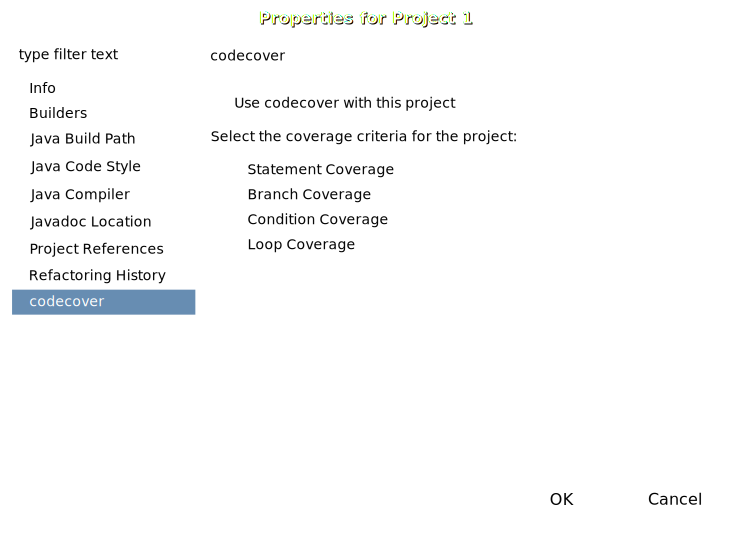
\includegraphics[width=1.0\textwidth]{images/Project_Configuration_Dialog/Project_Configuration_Dialog}
 \caption{Project properties dialog}
 \label{ui_fg:Project properties dialog}
\end{figure}

\newpage
%% \subsection{Test case notification} \label{ui:Test case notification}
%% The software extends the Eclipse menu \eclui{Source} and adds a new sub menu \eclui{\gbt Test Case Notification}. Therein new menu items are available:
%% \begin{itemize}
%%   \item \eclui{Start Test Case With Name And Comment}
%%   \item \eclui{Start Test Case With Name Only}
%%   \item \eclui{End Test Case With Name}
%%   \item \eclui{End Last Test Case}
%% \end{itemize}
%% \par
%% Also, corresponding templates are integrated to the Eclipse editor to allow easy inserting of the \gl[test case]{test case} notification statements described in section~\ref{fr:Test sessions and test cases}.

\subsection{Correlation Matrix}
\subsubsection{Mathematic prelude}\label{ui:Mathematic prelude}
The \eclui{Correlation Matrix} shows the correlation between test cases of a single test-session-container. Every test case contains a set of coverable items, which represents those parts of the code, that were covered during an execution of the instrumented system under test. Those sets are defined as follows: 
\begin{equation}
C_{T}:= \{ x | x \in T \wedge x \in CoverableItems \wedge x \in covered \}
\end{equation}

Correlation between two test cases $T_{1}$, $T_{2}$ is then defined as:
\begin{equation}
K_{U,V} := \frac{\mid U \cap V \mid}{\mid V \mid}
\end{equation}
with $U = C_{T_{1}}$ and $V = C_{T_{2}}$.
\par
Using this definition of correlation a \textit{partially ordered set} $R$ can be defined:
\begin{equation}
R = \{(U,V) \in C \times C : K_{U,V} = 1 \}
\end{equation}
In words this means, that two test cases $T_{1}$, $T_{2}$ are in relation $R$, if, and only if, $T_{1}$ contains all the coverable items $T_{2}$ does(or possibly more), which would make $T_{2}$ superfluous. This \textit{partially ordered set} then allows to detect and establish subsumption chains, in which one test cases completely contains another and so forth.
\par
Proof that $R$ is a \textit{partially ordered set} requires to proof that it possesses the following three attributes:
\begin{enumerate}
\item reflexivity
	\begin{equation}
	(U,U) \in R \Leftrightarrow \frac{\mid U \cap U \mid}{\mid U \mid} = 1 \Leftrightarrow \frac{\mid U \mid}{\mid U \mid} = 1
\end{equation}

\item antisymmetry
\begin{eqnarray}
	(U,V) \in R \Leftrightarrow \frac{\mid U \cap V \mid}{\mid V \mid} = 1 \Leftrightarrow V \subseteq U \\
	(V,U) \in R \Leftrightarrow \frac{\mid V \cap U \mid}{\mid U \mid} = 1 \Leftrightarrow U \subseteq V \\
\Rightarrow	V \subseteq U \wedge U \subseteq V \Rightarrow U = V
\end{eqnarray}

\item transitivity
\begin{eqnarray}
	(U,V) \in R \Leftrightarrow \frac{\mid U \cap V \mid}{\mid V \mid} = 1 \Leftrightarrow V \subseteq U \\
	(V,W) \in R \Leftrightarrow \frac{\mid V \cap W \mid}{\mid W \mid} = 1 \Leftrightarrow W \subseteq V \\
\Rightarrow	W \subseteq V \wedge V \subseteq U \Rightarrow W \subseteq U \Leftrightarrow \frac{\mid U \cap W \mid}{\mid W \mid} = 1 \Leftrightarrow (U,W) \in R
\end{eqnarray}

\end{enumerate}
with $T_{1}$, $T_{2}$ and $T_{3}$ being three test cases and $U = C_{T_{1}}$, $V = C_{T_{2}}$ and $W = C_{T_{3}}$.

\begin{figure}[hbt]
 \centering
 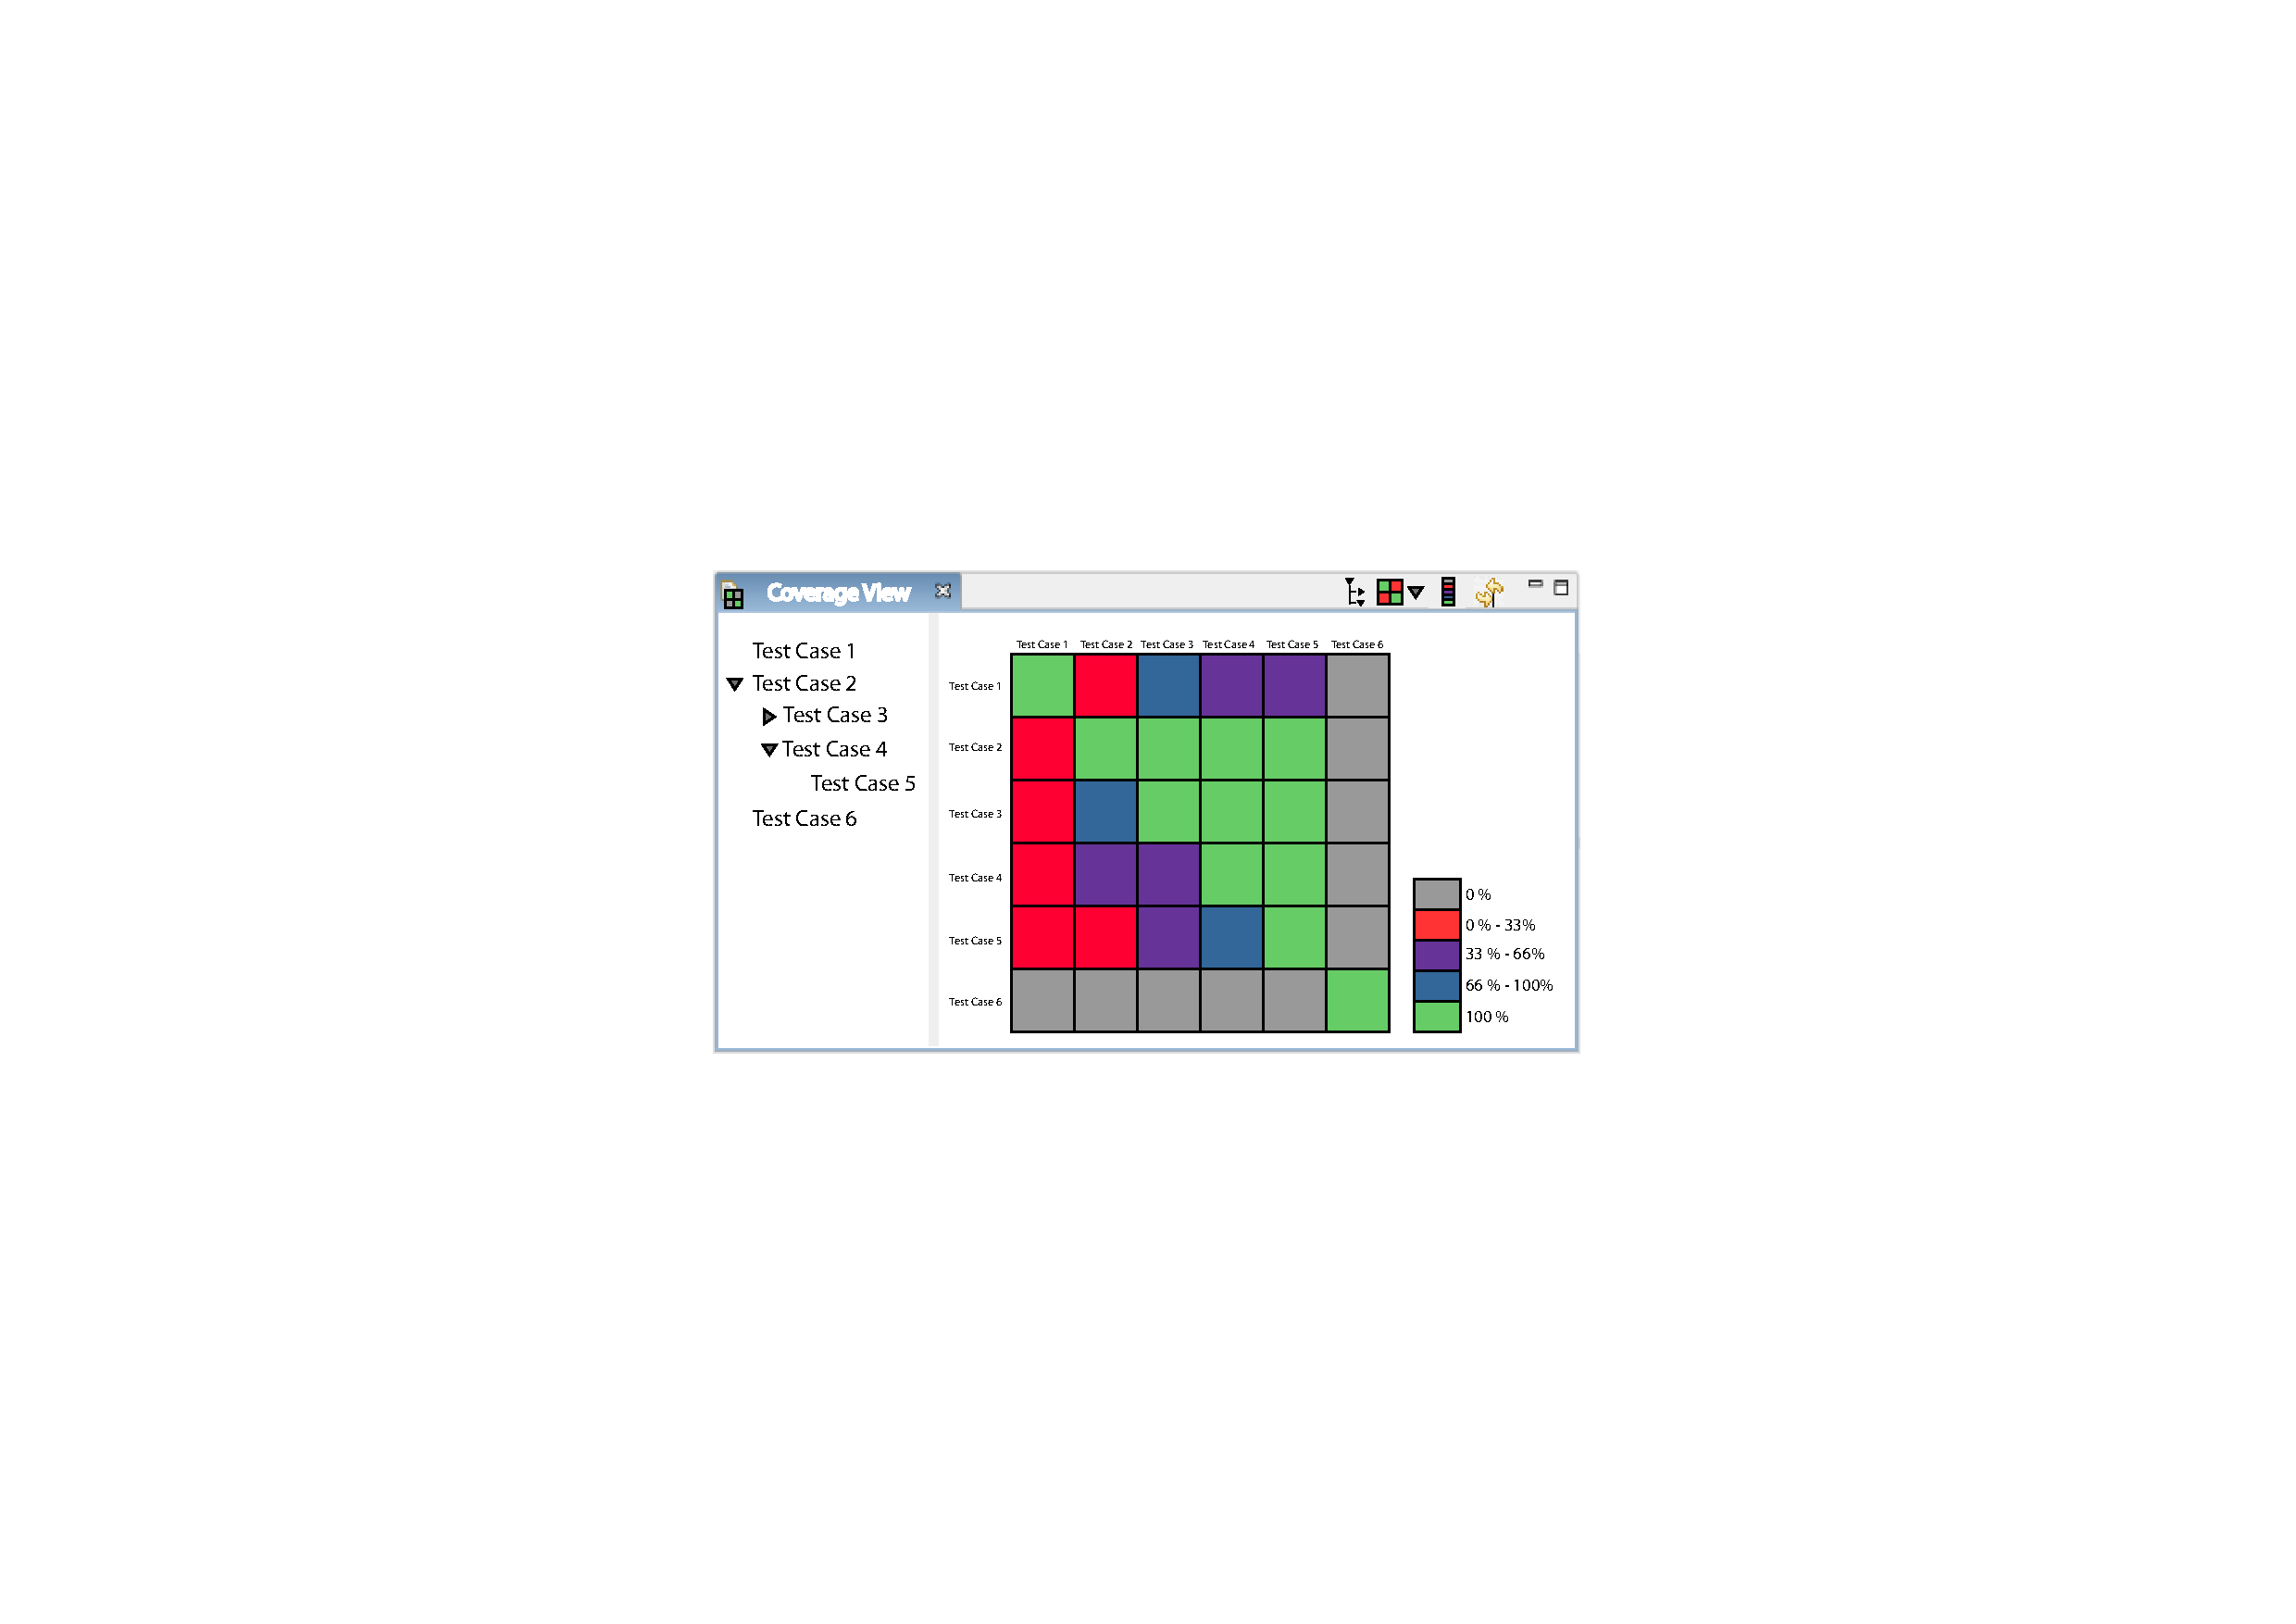
\includegraphics[width=1.0\textwidth]{images/Correlation_View/CorrelationView}
 \caption{Correlation View}
 \label{ui_fg:Correlation View}
\end{figure}
\subsubsection{Correlation View}
Using the definitions from \ref{ui:Mathematic prelude}, the view in Eclipse is defined as shown in figure~\ref{ui_fg:Correlation View}. A tree is located on the left of the view. This tree shows the subsumption chains of test cases defined in \ref{ui:Mathematic prelude}. All the children of a node in the tree are completely covered by the node itself.
\par	
The \eclui{correlation matrix} is located on the right side of the view. It shows all the test cases, that were used in the calculation of the correlation. The meaning of the colors is explained in the legend situated to the right of the matrix. The matrix is to be read from the left, e.g [test case left] covers [test case top] by [color value]\%. A tooltip shown, when hovering above one entry of the matrix, contains the exact percentage of correlation, as well as the amount of total coverable items and shared coverable items.
\par	
The tool bar items represent following commands (from left to right):
\begin{itemize}
\item Export the currently displayed matrix data into a .csv file - This command exports the data of the matrix into a comma seperated file.
\item Hide top-level tree items with no children - This command hides all the top level entries in the tree, which have no children, meaning they do not subsume any other test case;
\item Choose and calculate correlation - This command selects the metric to be used in calculating the correlation, with the pull-down menu of the arrow and calculates the correlation with a push on the button.
\item Show Legend - This command shows or hides the legend.
\item Automatically calculate correlation - If this command is toggled on, the correlation is automatically recalculated, when the selection of test case is changed. It can be switched off to improve performance.
\end{itemize}
\par
The test cases, that are to be used in the calculation, are selected using the \nameref{ui:Test sessions view}. If the \eclui{Automatically calculate correlation} command is toggled on, every change in the selection causes the correlation view to update its contents. Since this can potentially be time-consuming, the \eclui{Automatically calculate correlation} command can be toggled off and the \eclui{Choose and calculate correlation} command can be used, after the desired selection was achieved.


\subsection{Live Notification View}
\begin{figure}[hbt]
 \centering
 \includegraphics[scale=0.7]{images/Live_Notification/live_notification_view.png}
 \caption{Live Notification}
 \label{ui_fg:Live Notification}
\end{figure}
The \eclui{Live Notification View} is used to implement the \nameref{sec:fr:Live_Test_Case_Notification} (\ref{sec:fr:Live_Test_Case_Notification}). Two textfields are used to enter the hostname and port. The name of the test case can be entered as well. Test cases can be started and stopped with two labeled buttons. The test session can be finished with another button. The log file can be retrieved with the ``Download Coverage Log File'' button. This also automatically stores the data of log file in the test session container.

\subsection{Boolean Analyzer} \label{ui:Boolean Analyzer}
The \eclui{Boolean Analyzer} shows the boolean value of each basic boolean term, operator term and the root term according to evaluations of the condition which are recorded during the execution of the SUT. This data is presented in a table. The operators, operands and brackets define the columns and the evaluations are shown as rows in the table. In addition, a column for test cases is added. In that column one can see the test cases which covered the evaluation and the number of execution. 

Two table values of a column may contain green background. This represents that the basic boolean term of that column is covered according to the strict condition coverage criterion. If a column of a basic boolean term does not contain any colored values then the term is not covered. Figure \ref{ui_fg:Boolean Analyzer} shows the \eclui{Boolean Analyzer}.

\begin{figure}[hbt]
 \centering
 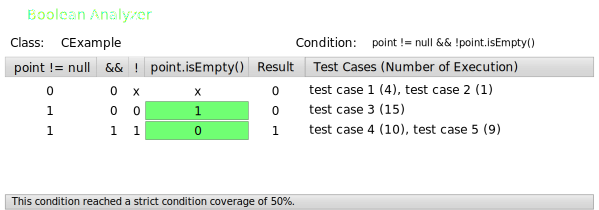
\includegraphics[width=1.0\textwidth]{images/Boolean_Analyzer/Boolean_Analyzer}
 \caption{Boolean Analyzer}
 \label{ui_fg:Boolean Analyzer}
\end{figure}

There are two ways to select a condition in the \eclui{Boolean Analyzer}. First, there are combo-boxes for classes and conditions. The second way is to select the keyword of the condition in the source code, right-click, and select the "Analyze Term" item in the context menu, which will automatically select the condition in the Boolean Analyzer.

\subsection{Hot-Path}\label{ui:Hot-Path}
The plugin displays line-wise execution counters corresponding to the currently selected test cases. The measured number of executions of lines is added to the \eclui{vertical ruler} of the java text editor via annotations with a color code. When the cursor hovers over such a Hot-Path annotation a tooltip with the execution counter is shown.

If no basic statement is found in a line, then no color is shown for that line in the ruler. Otherwise the color corresponding to the most often executed basic statement of that line is shown.

The color code is a mapping from the execution count of one line ($e$) and the highest exection count within a source file ($e_{max}$) to the color to mark that line. It must be encapsulated in a single method to make it easy to change in the source code. The mapping is a linear blending between the colors given in the users preferences. The exect mapping is: $color(e, e_{max}) = color_{max} * (e/e_{max}) + color_{null}(1-e/e_{max})$.

%%% Local Variables: 
%%% mode: latex
%%% TeX-PDF-mode: t
%%% TeX-master: "Specification.tex"
%%% End: 
